\documentclass[a4paper,12pt]{article} 

\usepackage[top = 2.5cm, bottom = 2.5cm, left = 2.5cm, right = 2.5cm]{geometry} 

% packages
\usepackage{amsmath, amsfonts, amsthm} % basic math packages
\usepackage{tikz} % for making illustrations
\usetikzlibrary{shapes.arrows, arrows, decorations.markings, positioning}
\usetikzlibrary{calc}
\usetikzlibrary{3d}
\usepackage{graphicx} % for importing images
\usepackage{xcolor} % more color options
\usepackage{colortbl}
\usepackage{multicol} % for making two-column lists
\usepackage{hyperref} % for hyperlinking
%\hypersetup{colorlinks=true, urlcolor=cyan,}
\usepackage{mathabx}
\usepackage{cleveref}
\usepackage{subfig}
\usepackage{array}
\usepackage{wrapfig}
\usepackage{bbm}
\usepackage{fancyhdr}
\usepackage{algorithm, algorithmicx, algpseudocode}
\usepackage{stmaryrd}
\usepackage{physics}


% The following two packages - multirow and booktabs - are needed to create nice looking tables.
\usepackage{multirow} % Multirow is for tables with multiple rows within one cell.
\usepackage{booktabs} % For even nicer tables.

% As we usually want to include some plots (.pdf files) we need a package for that.
\usepackage{graphicx} 

% The default setting of LaTeX is to indent new paragraphs. This is useful for articles. But not really nice for homework problem sets. The following command sets the indent to 0.
\usepackage{setspace}
\setlength{\parindent}{0in}

% Package to place figures where you want them.
\usepackage{float}

% The fancyhdr package let's us create nice headers.
\usepackage{fancyhdr}

% theorems, lemmas, examples, etc.
\newtheorem{theorem}{Theorem}[section]
% \newtheorem{corollary}{Corollary}[theorem]
% \newtheorem{lemma}[theorem]{Lemma}
\newtheorem{example}[theorem]{Example}
\newtheorem{lemma}[theorem]{Lemma}
\theoremstyle{definition}
\newtheorem{definition}{Definition}[section]
\theoremstyle{remark}
\newtheorem*{remark}{Remark}
\newtheorem*{solution}{Solution}

\def\mydefb#1{\expandafter\def\csname bf#1\endcsname{\mathbf{#1}}}
\def\mydefallb#1{\ifx#1\mydefallb\else\mydefb#1\expandafter\mydefallb\fi}
\mydefallb aAbBcCdDeEfFgGhHiIjJkKlLmMnNoOpPqQrRsStTuUvVwWxXyYzZ\mydefallb

\def\mydefb#1{\expandafter\def\csname cal#1\endcsname{\mathcal{#1}}}
\def\mydefallb#1{\ifx#1\mydefallb\else\mydefb#1\expandafter\mydefallb\fi}
\mydefallb aAbBcCdDeEfFgGhHiIjJkKlLmMnNoOpPqQrRsStTuUvVwWxXyYzZ\mydefallb

%% Change this to just the normal N,Z,R,C,P,E
\def\mydefb#1{\expandafter\def\csname bb#1\endcsname{\mathbb{#1}}}
\def\mydefallb#1{\ifx#1\mydefallb\else\mydefb#1\expandafter\mydefallb\fi}
\mydefallb CEGIKNPQRST\mydefallb

\newcommand{\half}{\frac{1}{2}}
\DeclareMathOperator{\sgn}{sgn}
\DeclareMathOperator*{\argmax}{arg\,max}
\DeclareMathOperator*{\argmin}{arg\,min}
\newcommand{\matlab}{\textsc{Matlab}}


%%%%%%%%%%%%%%%%%%%%%%%%%%%%%%%%%%%%%%%%%%%%%%%%
% 3. Header (and Footer)
%%%%%%%%%%%%%%%%%%%%%%%%%%%%%%%%%%%%%%%%%%%%%%%%

% To make our document nice we want a header and number the pages in the footer.

\pagestyle{fancy} % With this command we can customize the header style.

\fancyhf{} % This makes sure we do not have other information in our header or footer.

\lhead{\footnotesize CS 581:  Homework  \# 2}% \lhead puts text in the top left corner. \footnotesize sets our font to a smaller size.

%\rhead works just like \lhead (you can also use \chead)
\rhead{\footnotesize Scott (mtscot4)} %<---- Fill in your lastnames.

% Similar commands work for the footer (\lfoot, \cfoot and \rfoot).
% We want to put our page number in the center.
\cfoot{\footnotesize \thepage} 

\begin{document}
	
	
	%%%%%%%%%%%%%%%%%%%%%%%%%%%%%%%%%%%%%%%%%%%%%%%%
	%%%%%%%%%%%%%%%%%%%%%%%%%%%%%%%%%%%%%%%%%%%%%%%%
	
	%%%%%%%%%%%%%%%%%%%%%%%%%%%%%%%%%%%%%%%%%%%%%%%%
	% Title section of the document
	%%%%%%%%%%%%%%%%%%%%%%%%%%%%%%%%%%%%%%%%%%%%%%%%
	
	% For the title section we want to reproduce the title section of the Problem Set and add your names.
	
	\thispagestyle{empty} % This command disables the header on the first page. 
	
	\begin{tabular}{p{15.5cm}} % This is a simple tabular environment to align your text nicely 
		{\large \sc CS 581:  High Performance Computing} \\
		Emory University \\ Spring 2025 \\ Prof. Tianshi Xu \\
		\hline % \hline produces horizontal lines.
		\\
	\end{tabular} % Our tabular environment ends here.
	
	\vspace*{0.3cm} % Now we want to add some vertical space in between the line and our title.
	
	\begin{center} % Everything within the center environment is centered.
		{\Large \bf Homework \# 2} % <---- Don't forget to put in the right number
		\vspace{2mm}
		
		% YOUR NAMES GO HERE
		{\bf Mitchell Scott}\\ (mtscot4) % <---- Fill in your names here!
		
	\end{center}  
	
	\vspace{0.4cm}
	
	%%%%%%%%%%%%%%%%%%%%%%%%%%%%%%%%%%%%%%%%%%%%%%%%
	%%%%%%%%%%%%%%%%%%%%%%%%%%%%%%%%%%%%%%%%%%%%%%%%
	
	% Up until this point you only have to make minor changes for every week (Number of the homework). Your write up essentially starts here.
	
	\section{Environment}
	\begin{enumerate}
		
		\item {\bf List the environment you used to run the code (Operating System, CPU, RAM, etc.) }. 
		
		\begin{solution}
			The local environment where I was running the code was on a 2022 MacBook Pro with Apple M2 chip, 8 GB of RAM running macOS Sequoia 15.3.1. 
		\end{solution}
	\end{enumerate}
	\section{Sequential Code}
	\begin{enumerate}
		\item The results, which are averages of five runs where the fastest and slowest are removed, are seen in Tab. \ref{tab:Seq}.
		\begin{table}[h]
			\centering
			\begin{tabular}{|c|l|l|l|l|}
				\hline
				\textbf{Trial}& \texttt{small.bin} & \texttt{medium.bin}  & \texttt{large.bin} & \texttt{huge.bin} \\
				\hline\hline
					1&  6.5834e-05  (\textbf{high})	& 0.000828625 (\textbf{low})&1.23898	(\textbf{low})&6.73952	\\
					2&   3.0208e-05	&0.00109362	 (\textbf{high})	&1.24350	&6.69056 (\textbf{low})	\\
					3&   3.0875e-05&0.0009965	&	 1.32917 (\textbf{high})&6.79279\\
					4&     2.8542e-05 (\textbf{low}) & 0.000983875	&	1.25815&6.71300\\
					5&    2.9375e-05	& 0.000959958	& 1.26216	&6.82485 (\textbf{high}) \\
					\hline
					Avg&  \textbf{3.01527e-5} &	\textbf{0.000980111}& \textbf{1.25460}	&\textbf{6.748437}\\
				\hline
			\end{tabular}
			\caption{Sequential Code for different file sizes. All are reported in seconds.}
			\label{tab:Seq}
		\end{table}
	\end{enumerate}
	\section{Parallel Code}
	\subsection{Run Time}
	\subsubsection{\texttt{small.bin}}
	The results for \texttt{small.bin} are given in table \ref{tab:small}.
		\begin{table}[h]
			\centering
			\begin{tabular}{|c|l|l|l|l|}
				\hline
				\textbf{Trial}& \textbf{1 thread (s)}  &\textbf{2 thread (s)}  &\textbf{4  thread (s)}  &\textbf{8 thread (s)}  \\
				\hline\hline
				1& 1.1875e-4 &1.60708e-4 &0.00127112  &  0.001822 (\textbf{low})\\
				2&  1.22291e-4 &1.74000e-4  &0.000373667  &  0.00222171\\
				3& 8.9958e-05 (\textbf{low})& 1.66537e-4 & 0.000272833 (\textbf{low}) &0.002149  \\
				4& 1.5875e-4 & 1.42042e-4 (\textbf{low}) & 0.00167750 (\textbf{high}) &0.00444679 (\textbf{high})\\
				5& 1.67583e-4  (\textbf{high})&1.82500e-4 (\textbf{high})  & 0.000644041  & 0.00199421 \\
				\hline
				Avg& \textbf{1.33264e-4} &\textbf{1.67082e-4} &\textbf{7.62943e-4} & \textbf{0.00212164}\\
				\hline
			\end{tabular}
			\caption{Time (s) to sort data in \texttt{small.bin} dataset for varying number of threads.}
			\label{tab:small}
		\end{table}

		
	
	\subsubsection{\texttt{medium.bin}}
		The results for \texttt{small.bin} are given in table \ref{tab:medium}.
	\begin{table}[h]
		\centering
		\begin{tabular}{|c|l|l|l|l|}
			\hline
			\textbf{Trial}& \textbf{1 thread (s)}  &\textbf{2 thread (s)}  &\textbf{4  thread (s)}  &\textbf{8 thread (s)}  \\
			\hline\hline
			1& 0.00123242 (\textbf{high})&0.00364746  (\textbf{high}) & 0.00293096  (\textbf{high})  & 0.00612125\\
			2&  0.00110038 &0.00269762 &0.00197646 &  0.00327346 (\textbf{low})\\
			3&0.00122571 & 0.00240858& 0.00184267  (\textbf{low}) &0.0141560  (\textbf{high})\\
			4&0.000960625 (\textbf{low}) & 0.00208879 (\textbf{low})  &  0.00202196 &0.00400771 \\
			5& 0.00100529  &0.00277246 &0.00209833  & 0.00410279 \\
			\hline
			Avg& \textbf{0.00111046} &\textbf{0.00262622} &\textbf{0.00203225} & \textbf{0.00474392}\\
			\hline
		\end{tabular}
		\caption{Time (s) to sort data in \texttt{medium.bin} dataset for varying number of threads.}
		\label{tab:medium}
	\end{table}
	\subsubsection{\texttt{large.bin}}
	The results for \texttt{large.bin} are given in table \ref{tab:large}.
	\begin{table}[h]
		\centering
		\begin{tabular}{|c|l|l|l|l|}
			\hline
			\textbf{Trial}& \textbf{1 thread (s)}  &\textbf{2 thread (s)}  &\textbf{4  thread (s)}  &\textbf{8 thread (s)}  \\
			\hline\hline
			1& 1.14397 &0.908378 (\textbf{low})&0.529193  (\textbf{low})& 0.534565(\textbf{low})\\
			2&  1.13633 &0.952551 (\textbf{high})& 0.534829  &  0.696034 (\textbf{high})\\
			3& 1.17768 (\textbf{high}) & 0.909059 & 0.532734 & 0.586798 \\
			4&1.1341 &0.914919 & 0.533748&0.576026\\
			5& 1.13208 (\textbf{low})&0.91012 & 0.543836  (\textbf{high}) & 0.607107\\
			\hline
			Avg& \textbf{1.13813} &\textbf{0.911366} &\textbf{0.533770} & \textbf{0.589977}\\
			\hline
		\end{tabular}
		\caption{Time (s) to sort data in \texttt{large.bin} dataset for varying number of threads.}
		\label{tab:large}
	\end{table}
	\subsubsection{\texttt{huge.bin}}
	The results for \texttt{huge.bin} are given in table \ref{tab:huge}.
	\begin{table}[h]
		\centering
		\begin{tabular}{|c|l|l|l|l|}
			\hline
			\textbf{Trial}& \textbf{1 thread (s)}  &\textbf{2 thread (s)}  &\textbf{4  thread (s)}  &\textbf{8 thread (s)}  \\
			\hline\hline
			1& 5.99075  (\textbf{high})&4.24292  (\textbf{low})&2.60889  (\textbf{low}) & 2.49775\\
			2&  5.96154 	&4.34822  &2.76255  (\textbf{high})&  2.54355  (\textbf{high})\\
			3& 5.88652  (\textbf{low})& 4.27647 & 2.61821 &2.34084 \\
			4& 5.94369 	& 4.40685   (\textbf{high})	& 2.69274 &2.25988  (\textbf{low}) \\
			5& 5.98632  &4.27752 & 2.71596 & 2.42781 \\
			\hline
			Avg& \textbf{5.96385} &\textbf{4.30074} &\textbf{2.67564} & \textbf{2.38880}\\
			\hline
		\end{tabular}
		\caption{Time (s) to sort data in \texttt{huge.bin} dataset for varying number of threads.}
		\label{tab:huge}
	\end{table}
	\subsection{Speedup}
	In terms of the speedup, first we need to recall that 
	\begin{align}
		\text{Speedup} = \frac{T_{\text{sequential}}}{T_{\text{parallel}}}\label{eqn:speedup}
	\end{align}
	So simply by dividing our times from the result in section 1, the speedup is seen in Tabs. \ref{tab:small}, \ref{tab:medium}, \ref{tab:large} and \ref{tab:huge}, we arrive at the speedup, which is seen in Tab. \ref{tab:speed}.
	\begin{table}[h]
		\centering
		\begin{tabular}{|c|l|l|l|l|}
			\hline
			\textbf{\# Threads}& \texttt{small} & \texttt{medium} & \texttt{large}   & \texttt{huge}\\
			\hline\hline
			1&  0.2263 & 0.8826 & 1.1023 & 1.1316 \\
			2&   0.1805 & 0.3732 & 1.3766 & 1.5691\\
			4&   0.0395 & 0.4823 & 2.3504 & 2.5222\\
			8&   0.0142 & 0.2066 &2.1265 & 2.8250\\\hline
		\end{tabular}
		\caption{Speedup of different data sets for varying number of threads.}
		\label{tab:speed}
	\end{table}
	
	This data is also presented in Fig. \ref{fig:speedup}. As we can see from both the figure and the table, we have no great speedup for any number of processors with the \texttt{small} and the \texttt{medium} dataset. This is due to the parallel overhead and message transferring, which isn't worth it at this size. However, for the \texttt{large} and the \texttt{huge} dataset, we see advantages for using the parallel code. Another note is the large dataset is only large enough for 4 processors to make sense to be used. It is large enough for some speedup but not too large to justify the extra communication costs that 8 have.
	\begin{figure}
		\centering
		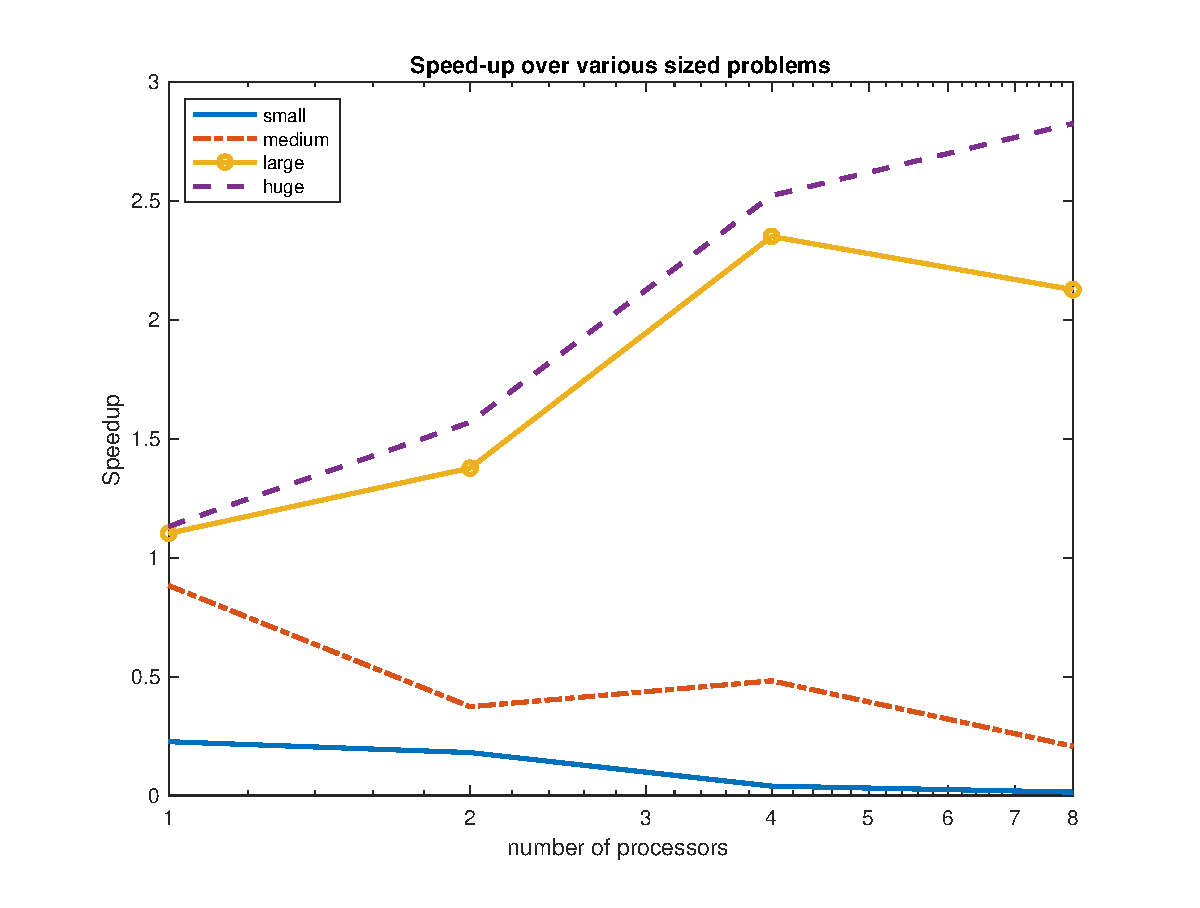
\includegraphics[width=0.8\linewidth]{speedup}
		\caption{Comparing the speedup curves for different datasets.}
		\label{fig:speedup}
	\end{figure}
	
	
	\subsection{Data Splits}
	Ideally, we would split the data in such a way that all processors get the same amount of data to sort locally, but since we don't know the distribution of the data, we cannot \textit{a priori} know the best splitting vector. Instead, we 
	\begin{figure}[h]
	\centering
	\includegraphics[width=0.45\linewidth]{dataSplits2}
	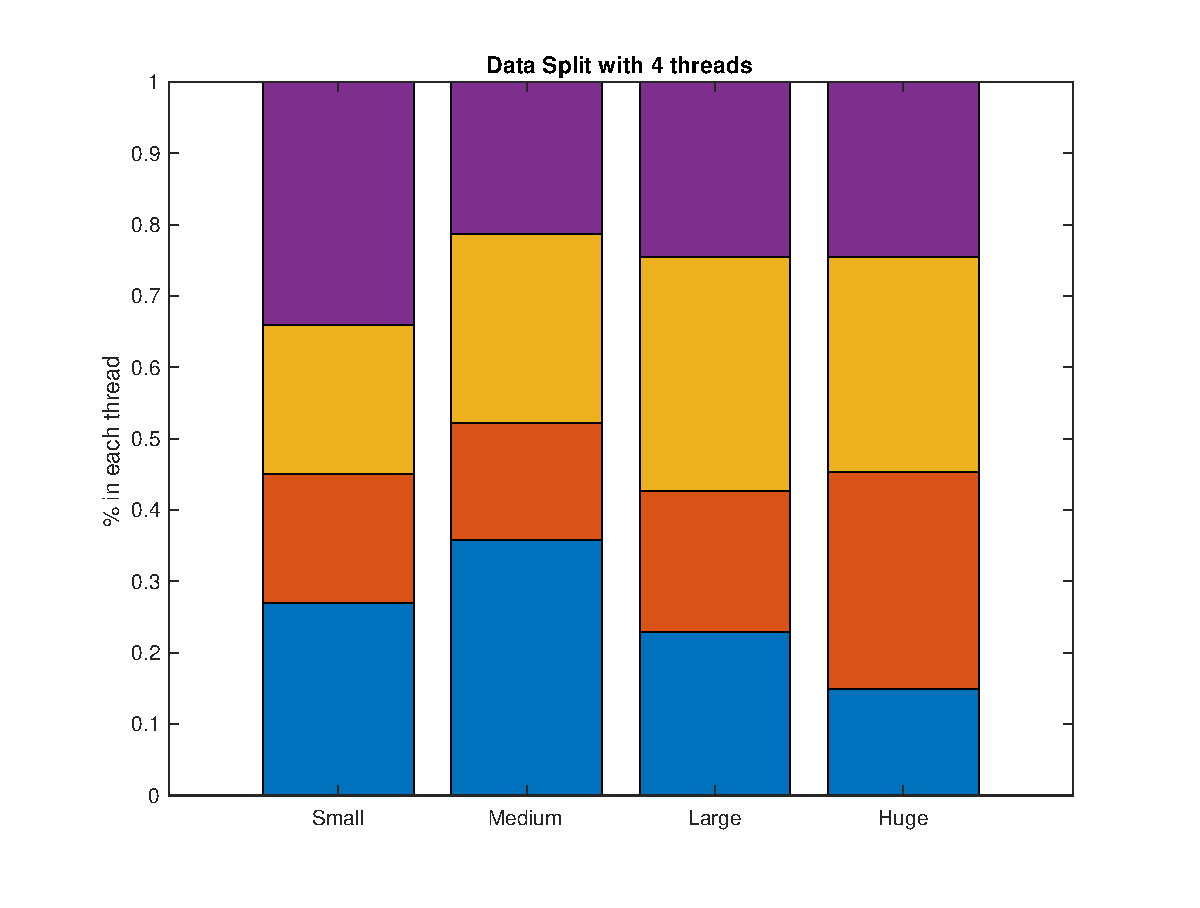
\includegraphics[width=0.45\linewidth]{dataSplits4}
	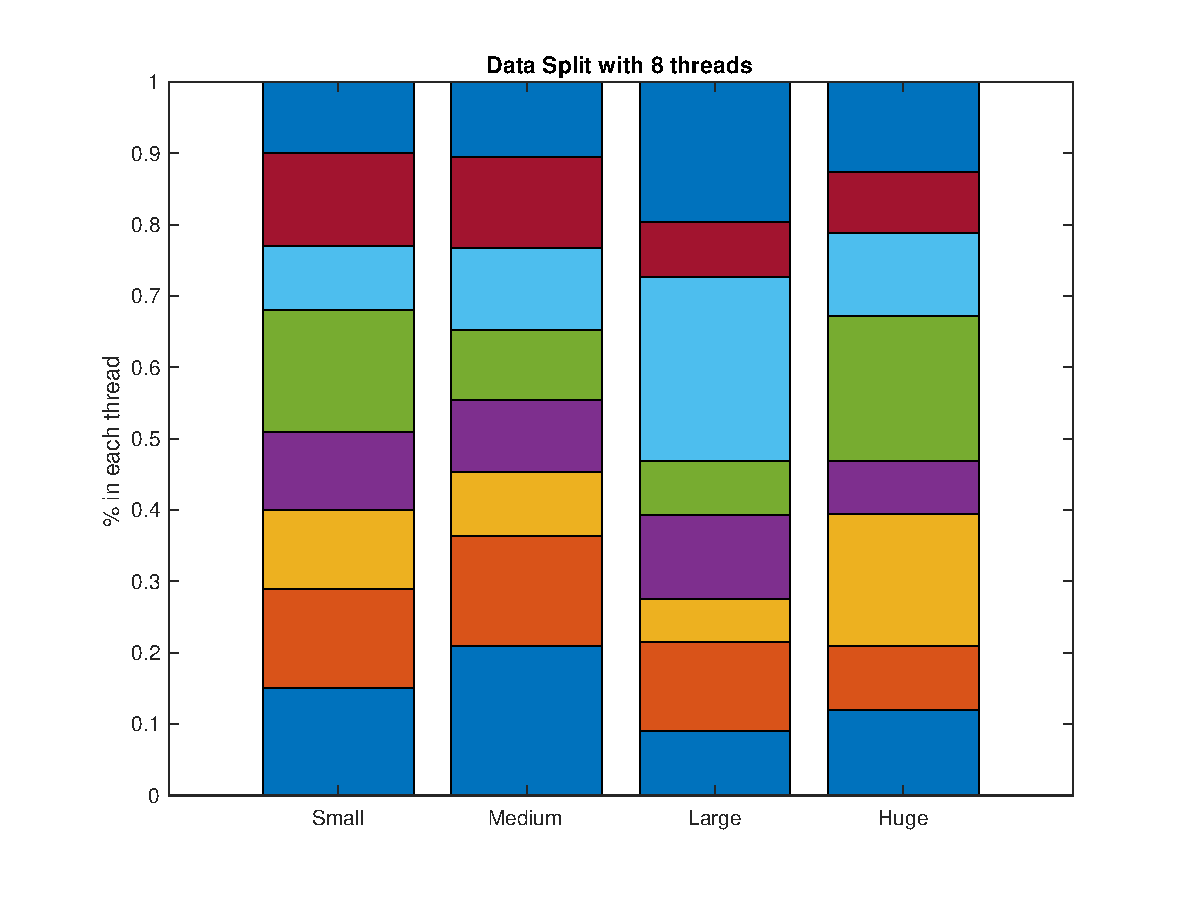
\includegraphics[width=0.45\linewidth]{dataSplits8}
	\label{fig:SpectralDeriv2}
	\caption{Visualized the data splits between processors for all datasets using (a) 2 threads, (b) 4 threads, and (c) 8 threads.}
	\end{figure}
	
	\section{Implementation}
	\begin{enumerate}
		\item \textbf{ Explain the Algorithm you used.}
		\begin{solution}
		
		\end{solution}
		\item \textbf{What is the performance bottleneck of your parallel implementation?}
		\begin{solution}
			
		\end{solution}
	\end{enumerate}
	
	
	
	\section*{Acknowledgements}
	I would like to acknowledge that I worked with fellow CS 581 students Emma Hart in OH on 2-4-25. Additionally I did use the Github Copilot to expedite my code (of course I checked the work it produced before I ran it). Lastly, I use resources from the University of Michigan EECS department to figure out how to structure my PThread code.
	
\end{document}
